\documentclass[journal]{IEEEtran}

\def\P(#1){\Phelper#1|\relax\Pchoice(#1)}
\def\Phelper#1|#2\relax{\ifx\relax#2\relax\def\Pchoice{\Pone}\else\def\Pchoice{\Ptwo}\fi}
\def\Pone(#1){\Pr\left( #1 \right)}
\def\Ptwo(#1|#2){\Pr\left( #1 \mid #2 \right)}
\def\Pr{\mathbf{Pr}}

\usepackage[utf8]{inputenc}
\usepackage{graphicx}
\usepackage{amsmath}
\usepackage{amsthm}
\usepackage{amssymb}
\usepackage{hyperref}
\usepackage{subfig}
\usepackage{multirow}
\usepackage[section]{placeins}

\usepackage{tabularx,booktabs}
\newcolumntype{C}{>{\centering\arraybackslash}X} % centered version of "X" type
\setlength{\extrarowheight}{1pt}
\usepackage{lipsum}
\usepackage[table]{xcolor}

\renewcommand\thesection{\arabic{section}}


% correct bad hyphenation here
\hyphenation{op-tical net-works semi-conduc-tor}


\begin{document}
\title{Python Stack Overflow Q$\&$A Analysis}
\author{Akanksha~Dwivedi(MT2016006)
        and~Tarini~Chandrashekhar(MT2016144),~\IEEEmembership{International Institute of Information Technology, Bangalore}}% <-this % stops a space

% The paper headers
\markboth{Machine Learning Project Report, \today}%
{Shell \MakeLowercase{\textit{et al.}}: Bare Demo of IEEEtran.cls for IEEE Journals}

\IEEEspecialpapernotice{(Draft Paper)}

% make the title area
\maketitle

% As a general rule, do not put math, special symbols or citations
% in the abstract or keywords.
\begin{abstract}
Stack Overflow has a vast amount of untapped potential in the form of questions and answers, asked and answered by and large by an active community of users. Not only do these questions give us an idea of problems encountered by the students taking on a particular \textbf{platform/technology}, but also give us a hint about the trend change, if any, over time. Here, we take a subset out of the questions and answers and focus on a single problem, Python. W explore trends and patterns in the questions asked by the students throughout the course of 8 years, i.e. 2008-2016. Second, the more challenging part of the problem is to make a \textbf{knowledge base from the questions/answers asked/answered by the users}. Now, using that knowledge base, we try to design a novel \textbf{course structure} in Python for students, using various Natural Language Processing techniques, which decide the feasibility of such an endeavour by comparing the summarized topics with a preexisting dictionary as well as modeling the topics in the form of a network graph, which aids in defining a hierarchy of topics.
\end{abstract}

% Note that keywords are not normally used for peerreview papers.
\begin{IEEEkeywords}
Machine Learning, Latent Dirichlet Allocation, Topic Modelling, Exploratory Analytics, Clustering
\end{IEEEkeywords}

\IEEEpeerreviewmaketitle

\section{Introduction}
Stack Overflow is a repository of questions and answers, which has served the purpose of solving various questions related to programming and being the most trusted online community for developers to learn and share over a period of 9 years, ever since its advent. There has been varying trends pertaining to a particular programming language. We consider Python, because it's the most sought after programming language, now-a-days, for data science and otherwise. Now, taking into account the active peer contribution for answering python-related questions; we can tap into these answers, to build a knowledge base, which could eventually help us design a course in python - A course which would be better informed by student's doubts and their trials and tribulations regarding the language. Our work focuses on following a set of methods which models the data into into topics, where each topic would be a collection of the most frequently occurring terms in that topic. Following this, we venture into exploring relationships between these topics. A course has topics which are interrelated, and not independent on their own. So, just modelling the questions and answers into topics would not be enough. We examine the relationship and closeness between the data, evaluate it, and then attempt to visualize it using various metrics and visualizations, respectively. In addition to this, we perform some standard analytics on the data, to render some trends about the users and the nature of questions and answers, in general.
The data is organized as three tables:
\begin{itemize}
    \item \textbf{Questions} contains the title, body, creation date, score, and owner ID for each Python question.
    \item \textbf{Answers} contains the body, creation date, score, and owner ID for each of the answers to these questions. The ParentId column links back to the Questions table.
    \item \textbf{Tags} contains the Id and the name of the Tag on the questions besides the python tag.
\end{itemize}
The dataset contains questions and answers satrting from 2nd Auguest,2008 up to 19 October,2016 (UTC).

\section{Related Work}
The algorithms/methodologies followed here, have been used on numerous textual datasets (online blogs, Google News, Wikipedia articles) available on the web. The StackLite dataset, consisting of Stack Overflow data of questions, answers and tags, was recently released publicly for performing various kind of analytics and discovering hidden trends in the data. A basic exploratory and descriptive analytics has already been performed to generate a brief summary of the data and to explore the popular tags, users, questions etc. Additionally, one of the work treats Stack Overflow data as a social network and follows a two-step process, using Natural Language Processing and KNN model fitting. It aims at: 
\begin{itemize}
    \item Finding the users who always ask the similar questions with the specific user.
    \item Finding the users who always provide similar answers with the specific user.
\end{itemize}
The former is analyzed with the questions data while the later uses the answers data. Before proceeding to the algorithm stage, the top 10000 users were selected in terms of the total number of questions and answers posted on the website, to be able to process the data with limited hardware and processing capabilities. Finally, different KNN models were built on the term frequency-inverse document frequency(tf-idf) table of the questions and answers dataset. The models then calculate the nearest neighbor of the user based on the question text and see which user also ask the same question. Silimar methodology was used to answer which users share the similar expertise in answering.

\section{Proposed Work}
We have applied the following algorithmic strategies on a subset of the dataset, i.e. questions and answers for the year 2008, as a Proof of Concept.

\subsection{Text Mining}
There are three different sub-datasets - questions, answers and tags. We perform exploratory data analytics on the questions, to forge a trend in the questions, asked in the python community. We find the patterns in the questions/answers repository, in order to get a better understanding of the topics that are asked more often as well as the questions which encourage relatively more debate and discussion. Similarly, the response rate on a question, in the form of score, also contributes in defining the difficulty level of the topic.
\subsection{Topic Modeling}
The second part of the analytics lies in charting a roadmap to design a \textbf{novel course structure in python from the repository of questions/answers} available on Stack Overflow. We plan on doing this by employing a variant of Topic Modeling on the data. On an abstract level, topic modeling helps us summarize large amounts of textual information by performing roughly, these three tasks :
\begin{itemize}
\item Discovering hidden topical patterns that are present across the collection.
\item Annotating documents according to these topics.
\item Using these annotations to organize, search and summarize texts.
\end{itemize}
Now, for the purpose of our problem statement, our corpus is a collection of about 8 million answers, which can be analogically treated as documents. Just as topic modelling is used to classify large amounts of documents into \textit{topic} or \textit{themes} which best represent the documents, we are going to generate topic models where topics are going to be the course content of Python. Now, in order to generate topic models, there are processes such as Latent Dirichlet Allocation(LDA) and its variants, and TextRank/LexRank process: graph-based algorithms to extract relevant key phrases for single/multi-document summarization.  
\vspace{0.5cm}

\subsubsection{LDA}
Latent Dirichlet Allocation(LDA) is a theme that facilitates \textit{automatic discovery of themes} in a collection of documents. The basic assumption behind LDA is that each of the documents in a collection consist of a mixture of collection-wide topics. However, in reality we observe only documents and words, not topics – the latter are part of the hidden (or latent) structure of documents. The aim is to infer the latent topic structure given the words and document. LDA does this by recreating the documents in the corpus by adjusting the relative importance of topics in documents and words in topics iteratively, by computing the probability that topic t generated word w as
\begin{equation}
    \P(t | w) = \P(t | d) * \P(w | t)
\end{equation}
where $\P(t | w)$ is the the proportion of words in document d that are currently assigned to topic t and $\P(w | t)$ is the proportion of assignments to topic t over all documents that come from this word w. 

The term 'Dirichlet' in LDA comes from the assumption that words and topics usually follow Dirichlet Distributions. Dirichlet distributions provide good approximations to word distributions in documents and, perhaps more importantly, are computationally convenient.
\vspace{0.5cm}

\subsubsection{TextRank/LexRank}
TextRank is an unsupervised, graph-based ranking model for keyword and sentence extraction. The basic idea of TextRank is to provide a score for each sentence in a text, taking the top-n sentences and sort them as they appear in the text, to build an automatic summary. A graph-based ranking algorithm is a way of deciding on the importance of a vertex within a graph, by taking into account global information recursively computed from the entire graph, rather than relying only on local vertex-specific information. The model is based on the concept of “voting” or “recommendation”. When one vertex links to another one, it is basically casting a vote for that other vertex. The higher the number of votes that are cast for a vertex, the higher the importance of the vertex. Moreover, the importance of the vertex casting the vote determines how important the vote itself is, and this information is also taken into account by the ranking model. Hence, the score associated with a vertex is determined based on the votes that are cast for it, and the score of the vertices casting these votes. Thus, knowledge drawn from an entire text is used in making local ranking/selection decisions. 
LexRank works somewhat on the similar lines as that of the TextRank. While TextRank uses a very similar measure based on the number of words two sentences have in common (normalized by the sentences' lengths), LexRank uses cosine similarity of TF-IDF vectors. Another important distinction between the two is that TextRank is used for single document summarization, while LexRank has been applied to multi-document summarization. The task remains the same in both cases—only the number of sentences to choose from has grown.
\vspace{0.5cm}

\subsection{Clustering}
Cluster analysis or clustering is the task of grouping a set of objects in such a way that objects in the same group (called a cluster) are more similar (in some sense or another) to each other than to those in other groups (clusters). Cluster analysis itself is not one specific algorithm, but the general task to be solved. It can be achieved by various algorithms that differ significantly in their notion of what constitutes a cluster and how to efficiently find them. Popular notions of clusters include groups with small distances among the cluster members, dense areas of the data space, intervals or particular statistical distributions.
A common problem when analysing large collections of documents is to categorize them in some meaningful way. This is easy enough if one has a predefined classification scheme that is known to fit the collection (and if the collection is small enough to be browsed manually). One can then simply scan the documents, looking for keywords appropriate to each category and classify the documents based on the results. More often than not, however, such a classification scheme is not available and the collection too large. One then needs to use algorithms that can classify documents automatically based on their structure and content. The basic idea behind document or text clustering is to categorise documents into groups based on likeness. 
The two types of clustering algorithms explored are:
\begin{itemize}
    \item \textbf{Hierarchical Clustering:} Connectivity based clustering, also known as hierarchical clustering, is based on the core idea of objects being more related to nearby objects than to objects farther away. These algorithms connect "objects" to form "clusters" based on their distance. A cluster can be described largely by the maximum distance needed to connect parts of the cluster. At different distances, different clusters will form, which can be represented using a dendrogram, which explains where the common name "hierarchical clustering" comes from: these algorithms do not provide a single partitioning of the data set, but instead provide an extensive hierarchy of clusters that merge with each other at certain distances. In a dendrogram, the y-axis marks the distance at which the clusters merge, while the objects are placed along the x-axis such that the clusters don't mix.
    \item \textbf{Centroid Based Clustering:} In centroid-based clustering, clusters are represented by a central vector, which may not necessarily be a member of the data set. When the number of clusters is fixed to k, k-means clustering gives a formal definition as an optimization problem: find the k cluster centers and assign the objects to the nearest cluster center, such that the squared distances from the cluster are minimized.
\end{itemize}

\section{Methodology}
\subsection{Exploratory Analytics}
Keeping the course design in mind, we explored the following questions to divide the course structure into descriptive session (which will require more active teaching by the mentor) and interactive sessions (inclining more towards an interactive classroom session).
\begin{itemize}
    \item Which were the most enquired topics/tags ?
    \item Which tags tend to have highest number of questions asked?
    \item Which tags tend to be most upvoted/downvoted on the basis of average scores?
    \item Which were the top N questions in a tag?
    \item Which tags tend to have highest number of answers?
    \item Which users answered the highest questions?
    \item Which users got the highest scores to their answers?
\end{itemize}
As explained above, we filtered out the questions and answers dataset for the year 2008. The questions, answers and tags data frames were merged into a single frame by the attributes question id and tags. Finally, all these questions were analyzed and answered from this new data set.

\subsection{Topic Modelling}
Topic Modelling broadly deals with classifying documents into themes. In our datasets, we deal with questions and answers separately, i.e. apply topic modelling to each separately. Topic modelling is often used as a text mining tool for discovering hidden structures in the data. In fact, topic model is a statistical model for discovering abstract topics that occur in the data. We use a topic model library to create a corpus from the dataset, and then remove all the extraneous information, such as punctuation, default stopwords in English, white spaces and eventually, convert all words to their root form. Having done this, we create a \textit{document term matrix} (DTM) which is a mathematical matrix that describes the frequency of terms that occur in a collection of documents. In a document-term matrix, rows correspond to documents in the collection and columns correspond to terms. This matrix becomes an input for the Latent Dirchlet Allocation that we performed next.
\vspace{0.5cm}

\subsubsection{Latent Dirichlet Allocation}
The LDA algorithm returns an object that contains a lot of information. Of particular interest to us are the document to topic assignments, the top terms in each topic and the probabilities associated with each of those terms. We can predefine the number of topics we want to be discovered from the dataset. Here, we have taken it as 40 for a corpus of approximately 1930 documents. We run the LDA function with the Gibbs Sampling option, which gives us a locally optimal solution, at best.

Gibbs sampling works by performing a random walk in such a way that reflects the characteristics of a desired distribution. Because the starting point of the walk is chosen at random, it is necessary to discard the first few steps of the walk (as these do not correctly reflect the properties of distribution). This is referred to as the burn-in period. We set the burn-in parameter to  4000. Following the burn-in period, we perform 2000 iterations, taking every 500th  iteration for further use.  The reason we do this is to avoid correlations between samples. We use 5 different starting points (nstart=5) – i.e. five independent runs. Each starting point requires a seed integer (this also ensures reproducibility),  so we have provided 5 random integers in our seed list. Finally we’ve set best to TRUE (actually a default setting), which instructs the algorithm to return results of the run with the highest posterior probability.

We can experiment with different values of number of topics, to find the best distribution of topics. 

\vspace{0.5cm}

\subsubsection{LexRank}
Each question/answer which is a part of the dataset, if analogized as a document, can be represented mathematically as point in a multidimensional space where the number of individual words in that document are the number of dimensions in that space. For example, if our document has three distinct words, it would be represented as (a,b,c) where a,b, and c are frequency of occurrence of the three distinct words in the document. Document similarity between two documents can be calculated as cosine similarity, which can broadly defined as the the dot product of the two document vectors. The vectors would be perpendicular in case of extreme dissimilarity, and parallel in case of being totally similar.
LexRank scores are calculated for node in a graph which has predefined number of nodes. Here, nodes are documents, and the LexRank scores are calculated by applying power method to the  quotient of cosine similarity matrix and the degree of each node. The power method is a standard iterative algorithm which helps Markov chain converge, by calculating the stationary distribution, by updating the eigen vector, on each iteration by multiplication with the stochastic matrix. it accounts for information subsumption among sentences. If the information content of a sentence subsumes another sentence in a cluster, it is naturally preferred to include the one that contains more information in the summary.

\begin{equation}
    p(u) = \frac{d}{N} + (1-d) \sum_{v\in \adj[u]}\frac{p(v)}{\deg(v)}
    
\end{equation}

\vspace{0.5cm}

\subsubsection{TextRank}
TextRank, like LexRank uses the concept of random walks and Eigen vector centrality. The edges between sentences are based on some form of semantic similarity or content overlap. While LexRank uses cosine similarity of TF-IDF vectors, TextRank uses a very similar measure based on the number of words two sentences have in common (normalized by the sentences' lengths). TextRank has usually been used for single-document summarizartion, whereas LexRank has been historically been used for multiple-document summarisation, so it applies a method to have no two similar documents in the top n nodes of the graph. TextRank applies no such filtering. 

\vspace{0.5cm}

\subsubsection{Clustering}
To apply the clustering algorithms, the filtered questions data of year 2008 was preprocessed to remove html tags, punctuations, control characters, special characters, whitespace and numbers. A corpus was constructed from this dataset, which was further transformed by removing common and custom stopwords and stemmed to convert words in their root forms. As the last step of pre-processing, the document-term matrix was constructed with length of words ranging from 5 to 10 and occurring in a minimum of atleast 1 document and not more than 1000 documents. This matrix was further processed to remove sparsity from the matrix. The strategies for hierarchical clustering fall into two types:
\begin{itemize}
    \item \textbf{Agglomerative}: where we start out with each document in its own cluster. The algorithm iteratively merges documents or clusters that are closest to each other until the entire corpus forms a single cluster. Each merge happens at a different (increasing) distance.
    \item \textbf{Divisive:} where we start out with the entire set of documents in a single cluster. At each step, the algorithm splits the cluster recursively until each document is in its own cluster. This is basically the inverse of an agglomerative strategy.
\end{itemize}
The algorithm we used is \textbf{hclust} which does agglomerative hierarchical clustering. After computing the distance matrix (i.e. computing the euclidean distance between observations), we run hclust algorithm with \textbf{Ward's Method}, in which the criterion for choosing the pair of clusters to merge at each step is based on the optimal value of an objective function. The results are visualized using dendograms.
In hierarchical clustering we did not specify the number of clusters upfront. To estimate the optimum number of clusters, we plotted the elbow curve, between the Within-cluster Sum of Squares (i.e. the sum of the distances between the points in a cluster and the cluster’s centroid) and the number of clusters . Actually, the quantity that is minimised is the total of the within-cluster sum of squares (WSS) between each point and the mean. Intuitively one might expect this quantity to be maximum when k=1 and then decrease as k increases, sharply at first and then less sharply as k reaches its optimal value.
The problem with this reasoning is that it often happens that the within cluster sum of squares never shows a slowing down in decrease of the summed WSS. Unfortunately this is exactly what happens in the case at hand.

\section{Results}
\subsection{Exploratory Analytics}
After performing the analysis, we observed that:
\begin{itemize}
    \item Among the list of most enquired topics/tags, \textbf{python} and \textbf{django} occupied the top positions with approximately 32$\%$ and 3$\%$ while \textbf{zementa}, \textbf{zipfile} and \textbf{zombie-process} occupied the lowest positions, each with 0.02$\%$.
    \item The highest number of questions (1927) were asked in the \textbf{python} tag with an average score of 54 while only 1 question was asked in \textbf{zementa}, \textbf{zipfile} and \textbf{zombie-process}.
    \item \textbf{coroutine} and \textbf{yield} tags had the most upvoted questions with an average score of 5524 and \textbf{python-2.1} and \textbf{clr} had the most downvoted questions with average score of -1 and -3.
    \item In the \textbf{python} tag, the top 3 questions found were:
    \begin{itemize}
        \item \textbf{What does the \textbf{yield} keyword do?}
        \item \textbf{What is a metaclass in Python?}
        \item \textbf{How do I check whether a file exists using Python?}
    \end{itemize}
    \item Similar to the former, \textbf{python} and \textbf{django} were the most popular in terms of number of users answering in the respective tags.
    \item The most popular users were the user \textbf{10661} answering 285 questions and the user \textbf{9493} answering 93 answers.
    \item User \textbf{9951} and user \textbf{1057} got the highest average scores in their answers.
\end{itemize}
\subsection{Topic Modelling}

\noindent The visualization results of topic modelling are shown with Term Occurrence histogram and WordCloud on the 2016 questions dataset. The x-axis of the term occurrence histogram are the terms in the corpus while y-axis gives the frequency of each of those terms. Only the terms of frequency more than 10000 are shown in the histogram.
\begin{figure}[!htb]
\begin{center}
\includegraphics[scale=0.15]{Term-Occurrence-Histogram.png}
\end{center}
\caption{Term Occurrence Histogram with frequency greater than 10000}
\end{figure}

\begin{figure}[!htb]
\begin{center}
\includegraphics[scale=0.25]{Wordcloud.png}
\end{center}
\caption{Wordclouds for word frequency greater than 1000}
\end{figure}

\noindent There are 1927 documents(questions) in total and there in we tune our LDA algorithm to discover 40 topics.
\begin{figure}[!htb]
\begin{center}
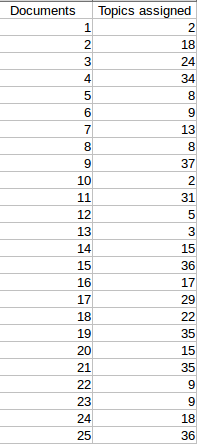
\includegraphics[scale=0.4]{DocsToTopics.png}
\end{center}
\caption{Questions to topics mapping where k(number of topics)=40 }
\end{figure}

\noindent The topics discovered in the documents are listed below with varying probabilities. These probabilities give us a hint about the importance of various topics for each document and hidden structure in questions/answers data.
\begin{figure}[!htb]
\begin{center}
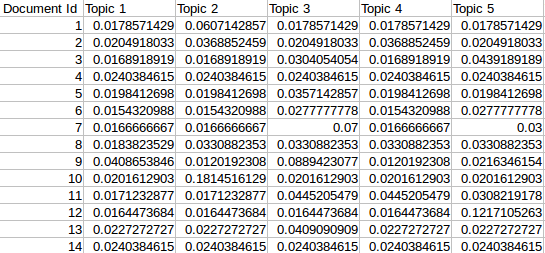
\includegraphics[scale=0.35]{ProbabilitiesAssociatedWithEachTopic.png}
\end{center}
\caption{Probabilities associated with each topic }
\end{figure}

\noindent We further explore the topics listed by enlisting the top terms as found out by the algorithm. We can gauge how accurate the algorithm is at inferring context by looking at how closely the terms listed come under a particular topic.
\begin{figure}[!htb]
\begin{center}
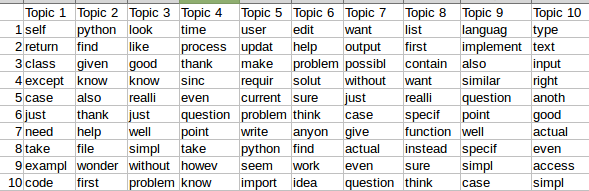
\includegraphics[scale=0.3]{Top10TermsInTopics.png}
\end{center}
\caption{Top 10 terms in topics}
\end{figure}

\noindent Additionally, the output of LDA algorithm is used to construct Document to Topic distribution matrix and Topic to Word distribution matrix. Posterior probabilities of topic t given word w, as defined above, are calculated from the former and a json object was created for visualization. The json object plots the inter-topic distance map for all k = 40 topics (given as input to LDA) and prints a histogram on the side, giving the distributions of top 30 most salient terms for each topic selected.

\subsection{LexRank}
 \begin{figure}[!htb]
\begin{center}
\includegraphics[scale=0.5]{LexRankScores.png}
\end{center}
\caption{The LexRank dataframe }
\end{figure}
\noindent The LexRank scores give us an idea of the most central page,or the most central document given a cluster of documents. 

\noindent The network graph constructed using open source software called Gephi, shows the cosine similarity among documents of a corpus. The vertices are the documents in the corpus while the edge denotes the association among documents. The node size is reflective of the connectivity of the node – i.e. the number of other documents to which it is cosine similar to varying degrees. The thickness of the edges reflect the degree of similarity among them.
\begin{figure}[!htb]
\begin{center}
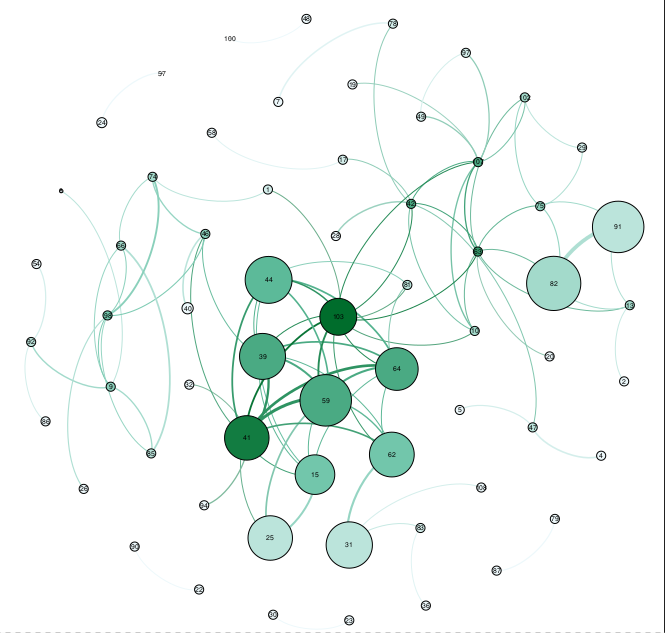
\includegraphics[scale=0.25]{Network_graph_ques_2008.png}
\end{center}
\caption{Network graph of 2008 questions corpus}
\end{figure}

\subsection{Clustering}
\noindent The results of clustering show that the 2008 questions dataset can be grouped in 4 clusters with each cluster representing the similar documents in terms of euclidean distance. The elbow plot between WSS and number of clusters also verifies our above claim with the elbow variation at k = 4, however the WSS still seems to decrease at a slower rate.
\begin{figure}[!htb]
\begin{center}
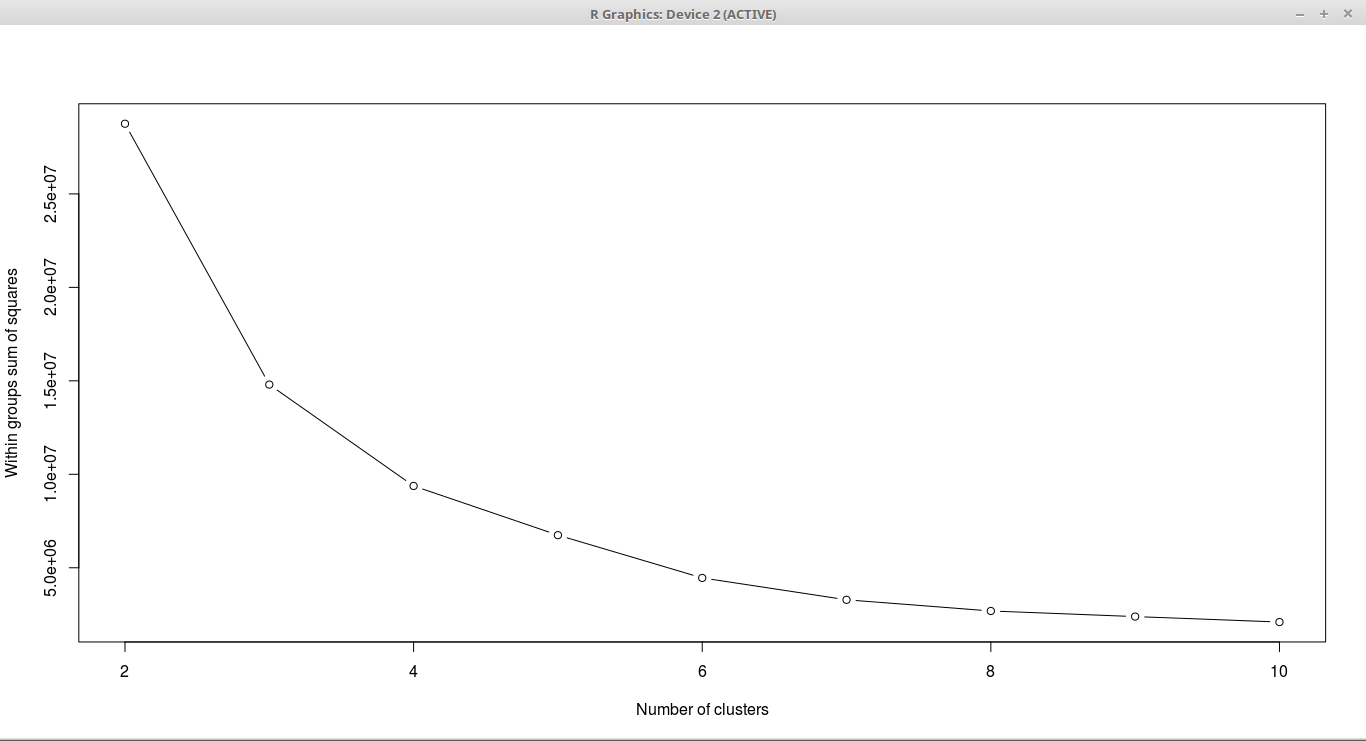
\includegraphics[scale=0.12]{Optimum_Clusters_using_Elbow_Method.png}
\end{center}
\caption{Optimum Clusters found using Elbow Curve between WSS and number of clusters (k)}
\end{figure}

\begin{figure}[!htb]
\begin{center}
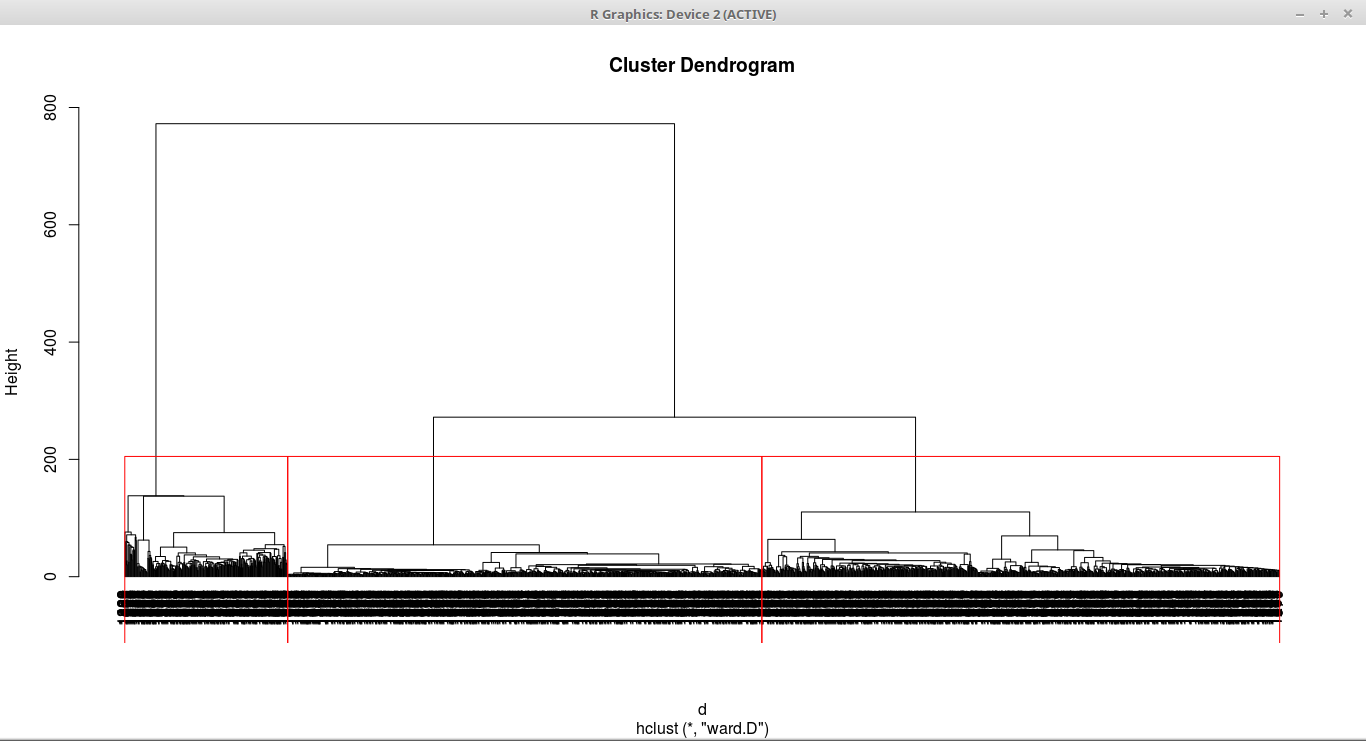
\includegraphics[scale=0.15]{Cluster_Dendogram_Groups_3.png}
\end{center}
\caption{Hierarchical Clustering with 3 clusters}
\end{figure}

\begin{figure}[!htb]
\begin{center}
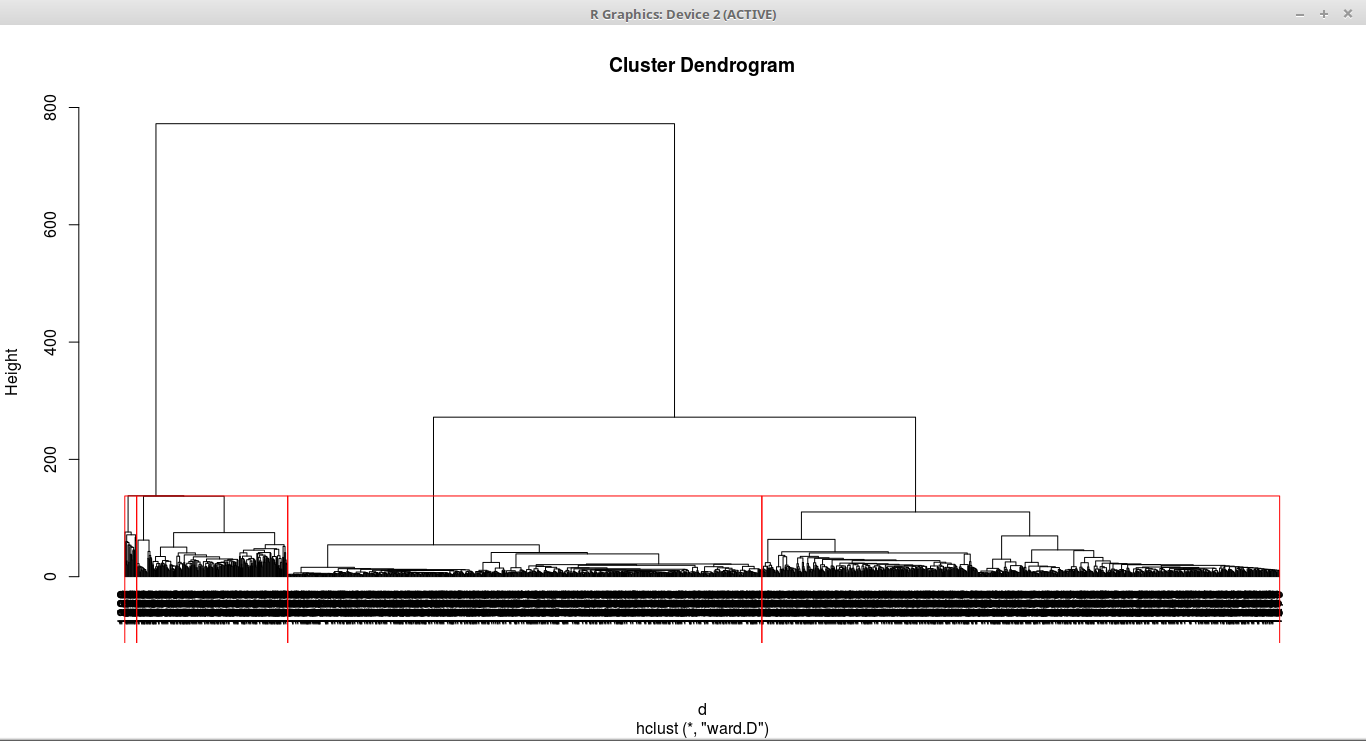
\includegraphics[scale=0.15]{Cluster_Dendogram_4_groups.png}
\end{center}
\caption{Hierarchical Clustering with 4 clusters}
\end{figure}

\section{Conclusion}
From the analytics done on the data, we gathered some insights about the data. The most popular tags/topics along with the top most questions in each tag can be given more focus than the other topics. Most answered questions could be included in the interactive sessions as most of the users are comfortable with them. From our application of LDA and Text Summarization algorithms like LexRank and TextRank, we are able to get a sense of the hidden structure in the form of topics in the data, and a similarity within them, which can be used for the course design. We have established closeness within the data by calculating cosine similarity matrices, as well as by clustering, which determines clusters based on the Euclidean distance between the questions/answers in the multidimensional space.


\section{Future Work $\&$ Improvements}
\begin{itemize}
\item In the present analysis, only the occurrence of tokens in a document, in the form of term frequency and inverse term frequency, has been taken in account. To bring out more semantic sense from the documents, the order of tokens can be taken in consideration for modeling long term dependencies in the dataset.
\item We can use deep learning models for better text summarization and eventually better dependency graphs. 
\item Since we have limited the work to a subset of dataset for the Proof of Concept, we can extend the trend analysis to subsequent years and document the change in the type of questions over a period of time.
\item We can improve the topic modelling by tuning the default parameters and tweaking the predefined number of topics.
\end{itemize}

\section*{Acknowledgment}
We would like to extend our gratitude to our Machine Learning course instructor, Prof. G. Srinivasaraghavan, whose invaluable guidance helped us build our intuition and gave our work a more academic perspective, rather than just being an exploratory analytics task.


\ifCLASSOPTIONcaptionsoff
  \newpage
\fi

\section{Data $\&$ Code}
\subsection{Data:} \url{https://www.kaggle.com/stackoverflow/pythonquestions}
\subsection{Code:} \url{https://github.com/tarini92/Python-QA-SO}

\begin{thebibliography}{1}
\bibitem{LexRank}
\url{https://www.cs.cmu.edu/afs/cs/project/jair/pub/volume22/erkan04a-html/erkan04a.html}
\bibitem{LDA}
\url{https://eight2late.wordpress.com/2015/09/29/a-gentle-introduction-to-topic-modeling-using-r/}
\bibitem{TextRank}
\url{https://web.eecs.umich.edu/~mihalcea/papers/mihalcea.emnlp04.pdf}
\bibitem{Topic Modelling}
\url{https://www.kdnuggets.com/2016/07/text-mining-101-topic-modeling.html}
\bibitem{Clustering}
\url{https://eight2late.wordpress.com/2015/07/22/a-gentle-introduction-to-cluster-analysis-using-r/}
\bibitem{Clustering-Wikipedia}
\url{https://en.wikipedia.org/wiki/Cluster_analysis}
\bibitem{Exploratory Analytics}
\url{http://www.analyticsforfun.com/2016/09/analyzing-stack-overflow-questions-and.html}

\end{thebibliography}

\end{document}
